\documentclass{article}
\usepackage[a4paper]{geometry}
\usepackage{amsmath}
\usepackage{hyperref}
\usepackage{amsfonts}
\usepackage{graphicx} % Required for inserting images
\usepackage{float}


\newcommand{\tm}{{\tau_{\mathrm{-}}}}
\newcommand{\tp}{{\tau_{\mathrm{+}}}}
\newcommand{\Var}{\mathrm{Var}}
\newcommand{\Med}{\mathrm{Med}}
\newcommand{\Prob}{\mathbb{P}}

\title{The Brownian Split method of Sampling Zero-free Intervals of a Brownian Bridge}
\author{Peter E. Creasey \\
  \href{https://orcid.org/0000-0002-4049-4928}{ORCID:0000-0002-4049-4928}}

\date{November 2024, last update Mar 2025}

\begin{document}

\maketitle

\section{Introduction}
\message{The cw \the\textwidth}

The zero-crossings of Brownian motion have long been of interest as a proxy for the time distribution of real-world events. Since the zeros are not isolated, however, direct simulation is usually only performed for a first hitting time (e.g. a L\'evy disribution), or the last zero in an interval (an arcsine law).

Here we describe the Brownian ``split'', which trisects a Brownian bridge into a bridge, excursion and bridge via sampling the last zero before the midpoint, and the first zero after. Such a procedure can be recursively applied until the intervals containing zeros (the bridges) have been trimmed to any desired length.

W.l.o.g. let us consider the standard bridge on the unit interval $W_t$, $t\in [0,1]$ whose endpoints are constrained to be $W_0=W_1=0$ and define $\tp,\tm$ to be the first zero after the midpoint and the last zero before, respectively. The main result here is that a method of jointly sampling $\tp,\tm$ is given by
\begin{eqnarray}
\tp &=& \frac{1}{1+\sin^2 \left( \frac{\pi}{2} U_1 \right)} \in \left(\frac{1}{2},1\right) \label{eq:stp} \\
\tm &=& \frac{U_2^2 \tp}{2\tp + U_2^2 -1} \in \left(0,\frac{1}{2}\right)  \label{eq:stm}
\end{eqnarray}
where $U_1,U_2$ are uniformly distributed random variables over $(0,1)$.
\begin{figure}[H]
\centering
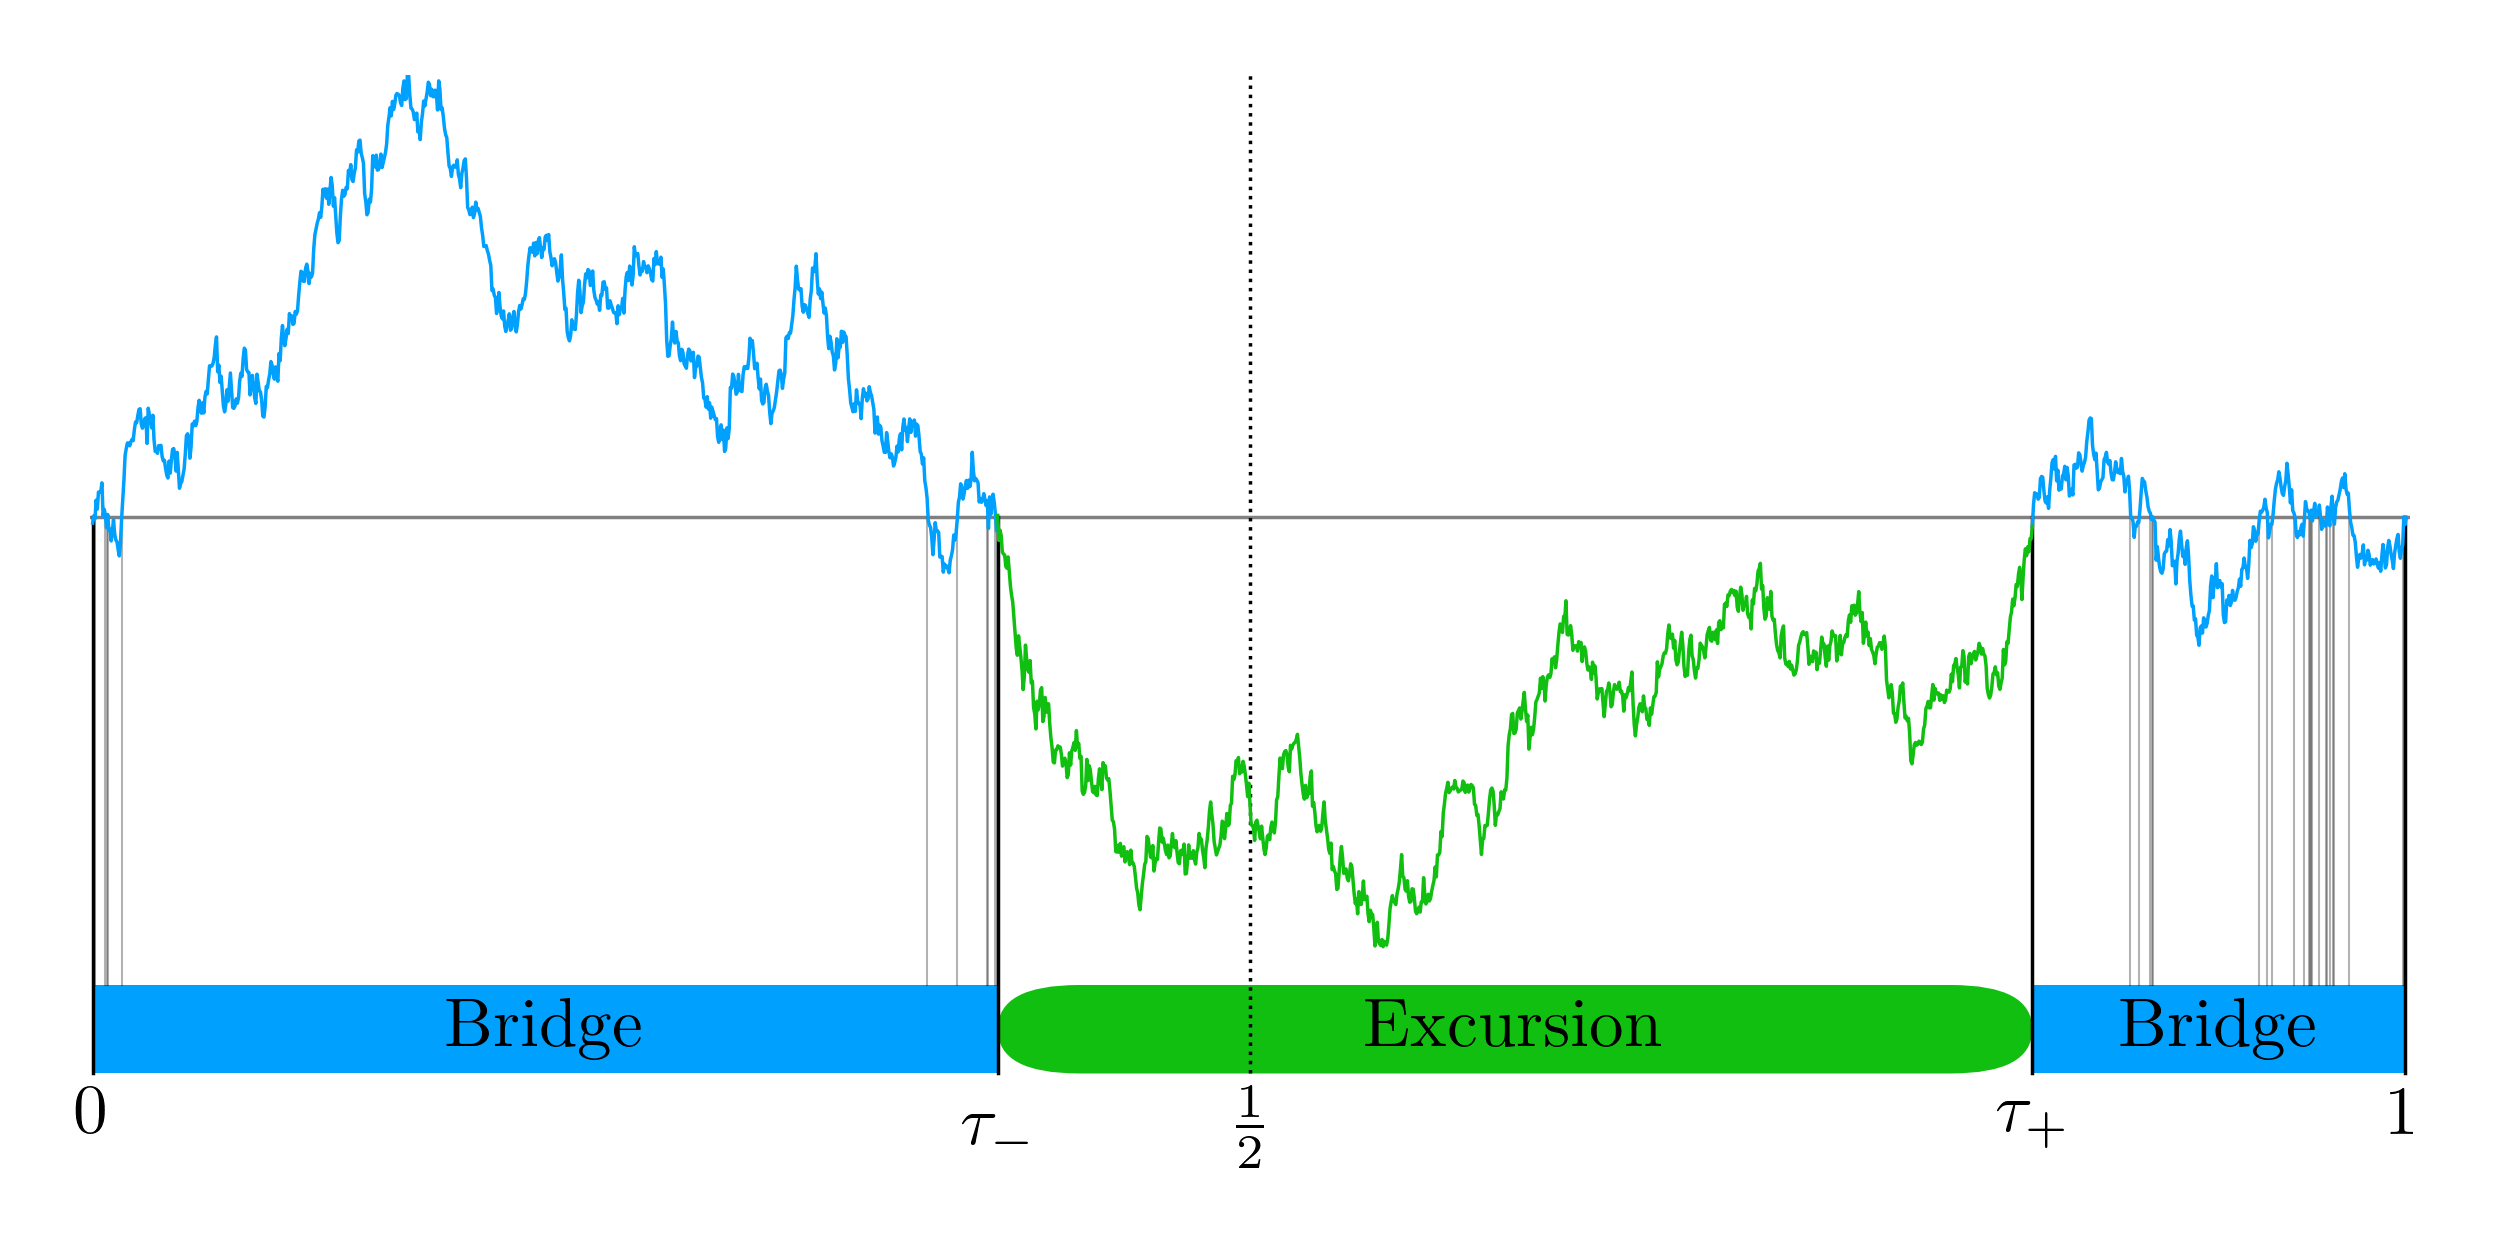
\includegraphics[width=\columnwidth]{figs/illustration.png}
\caption{Illustration of finding the last zero crossing ($\tm$) before the midpoint, and the first crossing after ($\tp$)}
\end{figure}

Some points of note are
\begin{itemize}
    \item{By construction $W_t$ forms a Brownian bridge over $[0,\tm]$, a positive/negative Brownian excursion over $[\tm,\tp]$, and then a Brownian bridge over $[\tp,1]$.}
    \item{The crossings $\tm$ and $1-\tp$ are identically distributed (but not independent). The median $\tp$ is $2/3$, and the mean is $\sqrt{1/2}$.}
    \item{The Pearson correlation between $\tm$ and $\tp$ is $-4/3 + \sqrt{8/9} \approx -0.39052$. This negative correlation can be intuitively understood by the clustering of zeros: a zero shortly before the midpoint (i.e. a large $\tm$) significantly increases the chances of a zero shortly after the midpoint (a small $\tp$), and vice-versa.}
\end{itemize}

\begin{figure}
\centering
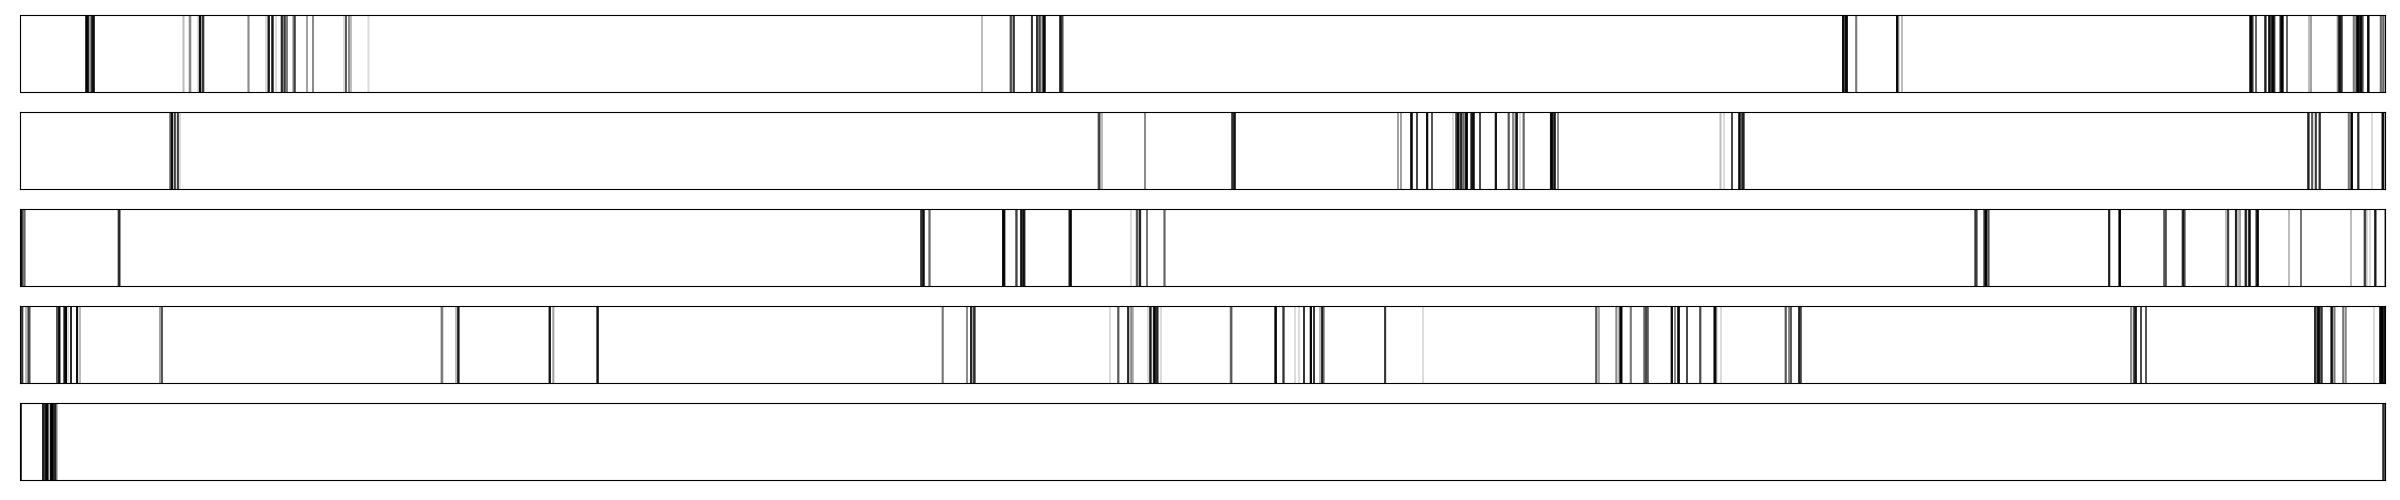
\includegraphics[width=\columnwidth]{figs/sample.png}
\caption{Example distributions of zeros (intervals recursively split until they are $<0.001\%$ of the original interval) using the sampling method in Eqns (\ref{eq:stp}-\ref{eq:stm})}
\end{figure}

\subsection{Brownian Split derivation}
We derive the above results, with a more general splitting point $\alpha \in (0,1)$. The approach here is to introduce the auxiliary variable $w=W_\alpha$, and then integrate over all $w$.

Let us define $\tp$ to be the first crossing of zero after $\alpha$. The barrier-hitting probability density of a walk starting at $W_\alpha=w$ \emph{without} the constraint at $W_1=0$ is given by the standard
\begin{equation}
\rho\left(\tp | W_\alpha=w\right) = \frac{|w|}{\tp - \alpha}\phi\left(w;\tp - \alpha \right) \, .
\end{equation}
where $\phi(x;\sigma^2)$ is the density of the normal distribution of zero mean and variance $\sigma^2$.
The density of arrival at $W_1=0$ is given by $\rho\left(W_1=0|W_\alpha=w\right) = \phi(w;1-\alpha)$, and similarly $\rho\left(W_1=0|\tp,W_\alpha=w\right) = \phi(0;1-\tp)$ (using the Markov property), and so by Bayes' theorem for densities we have
\begin{eqnarray}
  \rho\left(\tp | W_\alpha=w,W_1=0\right) &=& \frac{\rho(W_1=0|\tp,W_\alpha=w) \rho(\tp|W_\alpha=w)}{\rho(W_1=0|W_\alpha=w)} \\
&=&    \frac{|w|(1-\alpha)}{(\tp-\alpha)(1-\tp)}\phi\left(w;\frac{(1-\alpha)(\tp-\alpha)}{1-\tp}\right) \label{eq:tp_given_w} \,.
\end{eqnarray}
Noting that the probability density of $w$ is given by
\begin{equation}
\rho(w|W_1=0) = \phi\left(w;\alpha(1-\alpha)\right)
\end{equation}
(note we assume the condition $W_0=0$ for brevity) we can combine with (\ref{eq:tp_given_w}) to find the joint probability density of $\tp,w$ as
\begin{equation}\label{eq:tp_and_w}
  \rho(\tp,w|W_1=0) = \frac{|w|}{\tp-\alpha} \frac{1}{\sqrt{2 \pi (1-\tp)\tp}}\phi\left(w;\frac{(\tp-\alpha)\alpha}{\tp}\right)
\end{equation}
and we can integrate over $w$ as
\begin{eqnarray}
  \rho\left(\tp | W_1=0\right) &=& \int_{-\infty}^\infty {\textrm d}w   \rho\left(\tp,w | W_1=0\right) \\
&=&    \frac{1}{\pi \tp}\sqrt{\frac{\alpha}{(1-\tp)(\tp-\alpha)}} \label{eq:tp} \,.
\end{eqnarray}
(As an exercise for the reader, if we remove the Brownian bridge constraint $W_1=0$ and repeat this process we recover a L\'evy arcsine law \cite{levy}).
Integrating we can find the CDF
\begin{equation}
\textrm{CDF}\left(\tp | W_1=0 \right) = \frac{2}{\pi}\sin^{-1}\sqrt{\frac{\tp-\alpha}{(1-\alpha)\tp}}
\end{equation}
which can be inverted to find a sampling formula
\begin{equation}\label{eq:tp_sample}
\tp = \frac{\alpha}{\alpha + (1-\alpha) \sin^2 \left( \frac{\pi}{2} U_1 \right)} \in \left(\alpha,1\right)
\end{equation}
with $U_1$ a uniformly distributed random variable over $(0,1)$. The mean, variance and median are given by
\begin{eqnarray}
\mathbb{E}\left[\tp\right] &=& \sqrt{\alpha} \\
\Var\left[\tp\right] &=& \frac{1}{2}\sqrt{\alpha}\left(1-\sqrt{\alpha}\right)^2  \\
\Med\left[\tp\right] &=& \frac{2\alpha}{1+\alpha}  \, .
\end{eqnarray}

Now by symmetry w.r.t. time we find for the distribution of $\tm$ of the last zero before $\alpha$,
\begin{eqnarray}
\mathbb{E}\left[\tm\right] &=& 1-\sqrt{1-\alpha} \\
\Var\left[\tm\right] &=& \frac{1}{2}\sqrt{1-\alpha}\left(1-\sqrt{1-\alpha}\right)^2 \\
\Med\left[\tm\right] &=&  \frac{\alpha}{2-\alpha} \, .
\end{eqnarray}
and with (\ref{eq:tp_given_w}) we can find 
\begin{equation}
  \rho\left(\tm | W_\alpha=w\right) =  \frac{|w|\alpha}{\tm(\alpha-\tm)}\phi\left(w;\frac{\alpha(\alpha-\tm)}\tm\right) \label{eq:tm_given_w} \,.
\end{equation}
and combine with (\ref{eq:tp_and_w}) to give the joint density
\begin{equation}\label{eq:lwf}
\rho(\tm,w,\tp) = \frac{w^2}{2\pi} \frac{\phi\left(w;\frac{(\alpha-\tm)(\tp-\alpha)}{\tp-\tm}\right)}{(\alpha-\tm)(\tp-\alpha)\sqrt{\tm(1-\tp)(\tp-\tm)}} 
\end{equation}
(we omit the condition $W_1=0$ for brevity) and integrating over $w$
\begin{equation}\label{eq:tm_and_tp}
\rho(\tm,\tp) = \frac{1}{2\pi \sqrt{\tm(1-\tp)(\tp-\tm)^3}}
\end{equation}
then by Bayes (and the Markov property)
\begin{equation}
\rho(\tm|\tp) = \frac{\rho(\tm,\tp)}{\rho(\tp|W_1=0)} = \frac{\tp}{2} \sqrt{\frac{\tp-\alpha}{\alpha(\tp-\tm)^3\tm}}
\end{equation}
and integrate to the c.d.f.
\begin{equation}
  \textrm{CDF}(\tm|\tp) = \sqrt{\frac{(\tp-\alpha)\tm}{\alpha(\tp-\tm)}}
\end{equation}
to give a (conditional) sampling formula
\begin{equation}\label{eq:tm_sample}
\tm =  \frac{\alpha U_2^2 \tp}{\alpha U_2^2 + \tp - \alpha} \in \left(0,\alpha\right) \, .
\end{equation}

For the correlation we must perform a (fairly unpleasant) integral to find the moment
\begin{equation}\label{eq:tptm}
 \mathbb{E} \left[\tm\tp\right] =  \frac{1}{3} \left(2 + \alpha^{3/2} - \left(\alpha+2\right)\sqrt{1-\alpha}\right)
\end{equation}
which gives Pearson correlation coefficient
\begin{equation}\label{eq:corr}
 \mathrm{Corr} \left[\tm,\tp\right] =  \frac{2}{3} \frac{\left(1-\sqrt{\alpha}-\sqrt{1-\alpha}\right)}{\alpha^{1/4}\left(1-\alpha\right)^{1/4}}
\end{equation}

By splitting at the midpoint $\alpha=1/2$ into Eqs.~(\ref{eq:tp_sample}),(\ref{eq:tm_sample}) we recover the formulae in Eqs.~(\ref{eq:stp}-\ref{eq:stm}).

\section{Longest interval between zeros}

An interesting application of (\ref{eq:tm_and_tp}) is in terms of the longest interval between zeros of the Brownian bridge, a problem studied by \cite{wendel,godreche}. Denoting the longest the longest interval $l$, then if $l > 1/2$ then it is straightforward from the above analysis that this can only occur iff $\tp-\tm > 1/2$, and hence the cumulative probability is given by
\begin{equation}
  \mathbb{P}(l < r) = 2 - \sqrt{\frac{1}{r}}, \; r\in \left[ \frac{1}{2},1 \right]
\end{equation}
a result known to Ros\'en (via \cite{wendel}). 

For smaller values of $r$ the cumulative probability is only piecewise analytic \cite{godreche}, on the intervals $r^{-1} \in \left(n, n+1\right]$. Defining
\begin{equation}
  F_n(r) = \mathbb{P}(l < r), \; r^{-1} \in \left(n, n+1\right]
\end{equation}
then the $F_n$ can be written in terms of Wendel's factorial moments $M^\star_n$,
\begin{eqnarray}
  F_n(r) &=& \sum_{k=0}^n (-1)^k M^\star_k(r) \, . \label{eq:q_from_moment}
\end{eqnarray}
where $M^\star_n(r)$ is the expectation of $N(r) \choose n$, where $N(r)$ is the number of zero free intervals of length $> r$. The first of these is given by $M^\star_0(r) = 1$ and recurse to larger $n$ via Laplace transform,
\begin{equation}
  M^\star_{n+1}(r) = \begin{cases}
    \frac{1}{\pi} \int_{nr}^{1-r} \frac{{\rm d}x}{1-x} M^\star_n\left(\frac{r}{x}\right) \sqrt{\frac{1-r-x}{rx}}, & 0<r<\frac{1}{n+1}, \\
    0, & \text{otherwise}
    \end{cases}
\end{equation}
(note the lower limit in \cite{wendel} is given as zero rather than $nr$, however $M^\star_n(r)$ zero for $nr < 1$, so this is equivalent).

Application of this recurrence gives us straightforward expressions for 
\begin{eqnarray}
  M^\star_1(r) &=& \frac{1}{\sqrt{r}} - 1 \\
  M^\star_2(r) &=& \frac{2}{\pi}\left[\frac{\sqrt{1-2r}}{r} + \cos^{-1}\frac{r}{1-r}-\frac{2}{\sqrt{r}} \cos^{-1} \sqrt{\frac{r}{1-r}}\right]
\end{eqnarray}
after which the integrals are problematic.

\begin{figure}
\centering
\includegraphics[width=\columnwidth]{figs/integrand.png}
\caption{Diagrams of the decomposition of the integrand in Eqn.~(\ref{eq:l_split}) as a function of $1-\tm$ and $\tp$. \emph{Left} is the even recurrence in Eqn.~(\ref{eq:F_even}), \emph{right} the odd recurrences in Eqn.~(\ref{eq:F_odd}).}
\label{fig:integrand}
\end{figure}

An alternative approach to finding the cumulative probability of the longest interval is to recursively subdivide Brownian bridges via Eqns.~(\ref{eq:tm_and_tp}). Taking $l_{\mathrm{-}}$ to be the longest interval in $[0,\tm]$, and $l_{\mathrm{+}}$ to be the longest interval in $[\tp,1]$, we may write
\begin{eqnarray}
  F_{n}(r) &=& \int_{\frac{1}{2}-r}^{\frac{1}{2}} {\rm d}\tm \int_{\frac{1}{2}}^{\tm+r} {\rm d}\tp \Prob\left(l_\mathrm{-} < \frac{r}{\tm}\right)\Prob\left(l_\mathrm{+} <\frac{r}{1-\tp}\right) \rho(\tm,\tp) \label{eq:l_split}
\end{eqnarray}
where the integration domain is restricted, since $\tp-\tm > r$ excludes the longest interval being shorter than $r$.

Eqn.~(\ref{eq:l_split}) may be decomposed as in the diagrams in Fig.~\ref{fig:integrand} for even $2n$,
\begin{eqnarray}
  F_{2n}(r) &=& 2 \int_{nr}^{\frac{1}{2}} {\rm d}\tm \int_{1-nr}^{\tm+r} {\rm d}\tp F_n\left(\frac{r}{\tm}\right)F_{n-1}\left(\frac{r}{1-\tp}\right)\rho(\tm,\tp) + \nonumber \\
  && \int_{1-(n+1)r}^{nr} {\rm d}\tm \int_{1-nr}^{\tm+r} {\rm d}\tp F_{n-1}\left(\frac{r}{\tm}\right)F_{n-1}\left(\frac{r}{1-\tp}\right)\rho(\tm,\tp) + \nonumber \\
  && \int_{nr}^{\frac{1}{2}} {\rm d}\tm \int_{\frac{1}{2}}^{1-nr} {\rm d}\tp F_n\left(\frac{r}{\tm}\right)F_n\left(\frac{r}{1-\tp}\right)\rho(\tm,\tp)  \label{eq:F_even}
\end{eqnarray}
where we take the ``natural'' convention $F_0(r)=1$. Similarly for odd $2n+1$ we have
\begin{eqnarray}
  F_{2n+1}(r) &=& \int_{nr}^{\frac{1}{2}} {\rm d}\tm \int_{\frac{1}{2}}^{\min(\tm+r,1-nr)} {\rm d}\tp F_n\left(\frac{r}{\tm}\right)F_n\left(\frac{r}{1-\tp}\right)\rho(\tm,\tp) + \nonumber  \\
  && 2 \int_{\frac{1}{2}-r}^{nr} {\rm d}\tm \int_{\frac{1}{2}}^{\tm+r} {\rm d}\tp F_{n-1}\left(\frac{r}{\tm}\right)F_n\left(\frac{r}{1-\tp}\right)\rho(\tm,\tp) \label{eq:F_odd}
\end{eqnarray}

These integrals allow us to go slightly further than the Laplace transform approach, giving
\begin{eqnarray}
  F_1(r) &=& 2 - \sqrt{\frac{1}{r}} \\
  F_2(r) &=&  2 - \frac{1}{\sqrt{r}} + \frac{2}{\pi}\left[\frac{1}{r}\sqrt{1-2r}-\frac{2}{\sqrt{r}} \cos^{-1} \sqrt{\frac{r}{1-r}} + \cos^{-1}\frac{r}{1-r}\right] \\
  F_3(r) &=& \frac{2}{\sqrt{r}} + \frac{1}{\pi}\left[\frac{8}{r}\sqrt{1-2r}-\frac{3r+1}{r\sqrt{r}} + 8 \cos^{-1} \frac{r}{1-r} - \frac{16}{\sqrt{r}}\cos^{-1}\sqrt{\frac{r}{1-r}}\right]
\end{eqnarray}
before the we can integrate no further. Interestingly the correspondence implies the 3rd factorial moment will be (via Eqn.~\ref{eq:q_from_moment})
\begin{equation}
  M^\star_3(r) = F_2(r) - F_3(r) = \frac{3}{\sqrt{r}} - 1 + \frac{3r+1}{\pi r^{\frac{3}{2}}} - \frac{6}{\pi}\left[\frac{\sqrt{1-2r}}{r} - \sin^{-1}\frac{r}{1-r}  +\frac{2}{\sqrt{r}} \sin^{-1}\sqrt{\frac{r}{1-r}}\right] \, .
\end{equation}

\begin{thebibliography}{9}
\bibitem{levy} L\'evy, P 1940 {\it Compositio Mathematica} {\bf 7}
\bibitem{wendel} Wendel J G 1964 {\it Math. Scand.} {\bf 14} 21
\bibitem{godreche} Godr\'eche, C 2017 {\it Journal of Physics A: Mathematical and Theoretical} {\bf 50} 19    
\end{thebibliography}
\end{document}
